
\begin{savequote}[8cm]

    We hear a lot these days about genes and molecules, but how does one human brain, or one human being coordinate, or entrain, or resonate with another?  We may not realise it but we live in a world of coordination, at every level and every scale of endeavour.

  \qauthor{--- J. A. S. Kelso  \textit{Coordination and the Complimentary Nature} Presentation to the The New York Academy of Sciences - May 12, 2010}
\end{savequote}


%I do not see any way to avoid the problem of coordination and still understand the physical basis of life.
%\qauthor{--- H. H. Pattee  \textit{The role of instabilities in the evolution of control hierarchies} 1976}


\chapter{\label{chap:theory}A theory of social bonding through joint action}


\minitoc


In response to the knowledge gaps identified in the Introduction, in this chapter I outline a novel theory of social bonding through joint action, which will be tested in subsequent empirical studies of joint action among Chinese rugby players.  In particular, I identify team click as a special case phenomenon of joint action and a potential mediator of the relationship between joint action and social bonding in group exercise contexts.  Emerging research from the social cognition of joint action suggests that a continuum of cognitive mechanisms are responsible for establishing and maintaining behavioural coordination between two or more individuals.  More efficient solutions to the cognitive uncertainty of joint action appear to involve reducing the cognitive demands associated with interoceptive predictive modelling and instead increasing reliance on more direct extra-neural coupling with the environment.  These mechanisms also appear to be modulated by inter-individual and cultural variation in knowledge, expertise, experience, and personality type.  Evidence suggests coordination in joint action can set the foundation for social connection, and the phenomenon of team click can be understood as an optimal state of interpersonal coordination in joint action that maximally activates a causal pathway between joint action and social bonding.  I conclude the chapter by summarising a theory of social bonding through joint action, and outlining predictions that arise from this theory.




                                  \begin{CJK}{UTF8}{gbsn}

\section{Sun Hongwei, rugby's newest recruit\label{sect:SHW}}
Sun Hongwei arrived, escorted by his high school athletics coach, to the Beijing Temple of God of Agriculture Institute of Sport (hereafter the Institute) soon after I began my fieldwork in August 2015.  An 18-year-old with a slight build and timid demeanour---his gaze remained diverted to the ground during his first few months at the Institute---Hongwei later told me that he had never seen a rugby ball before that day he arrived.

Hongwei was from Hebei province, immediately surrounding the special prefecture of Beijing, China's capital.  As was relatively common practice at the time in the Chinese competitive sport system, Hongwei's coach had organised a trial for Hongwei with the Beijing Provincial Men’s and Women's Rugby Program (hereafter the Program) by calling upon social connections to the leadership of the Institute.

Athletes come to the Rugby Program from all over the country.  Representing Beijing at a provincial level in a sport like rugby can translate into the opportunity to gain entrance---via a designated ``specialist athlete'' (\textit{tiyu techan} 体育特产) pathway---to one of China's top universities (Beijing Sports University, in this case) and enhanced career employment opportunities thereafter.  Rugby is not a popular sport in China.  It is referred to as a neglected branch of the Chinese sport system, or a ``cold-gate'' (\textit{lengmen xiangmu} 冷门项目), referring to a profession, trade or branch of learning that receives little attention.  Despite its minnow status in China in terms of its popularity, rugby's recent inclusion in the Olympics (in the form of the modified seven-a-side version of ``rugby sevens'') means that it now occupies a prominent place in the Chinese sport system, which has been defined since its inception by a strong Olympic logic \citep{Brownell2008}.  If a sport is a current member of the summer or winter Olympic Games, then the sport is included in the roster of sports played at the quadrennial China National Games (\textit{quanhunhui}).  As such, rugby programs such as the one at the Institute now exist in twelve of China's 34 provincial level regions, either embedded within, or somehow associated with, tertiary education institutions.  Thus, although rugby and China are two words that have not historically featured within the same utterance, rugby in China now affords athletes a rare and under-capitalised opportunity to pursue attractive life-course opportunities of education and employment in an intensely competitive education system.

Without exception, the athletes who arrive at the Institute to join the rugby team have not spent their childhoods playing rugby in their schoolyards or watching professional rugby on television. Many who come to rugby transition from other more popular sports such as athletics, basketball, or association football, and often---like Hongwei---have never seen a rugby ball before they arrive.  Most ``start from scratch,'' so to speak, in terms of their grasp of the requirements of the highly interactive and technically complex team sport. In addition to complex patterns of movement coordination, rugby also involves unrestrained body-on-body collisions and intense bouts of high physiological exertion, requiring speed, strength, agility, and endurance to perform all of rugby's technical requirements successfully.  Learning the game of rugby from a baseline of essentially zero, while also navigating the inevitably demanding  social and political dynamics within the team and the Institute, was clearly going to be a daunting task for Hongwei.

                        \begin{center}
                          * * *
                        \end{center}

Hongwei was the first of the Program’s new recruits that I followed closely.  Even compared to other newly arrived junior athletes, he was noticeably timid and shy, particularly in his interactions with the coaches (myself included) and senior players. Nevertheless, Hongwei clearly signalled diligence and commitment through his participation in team activities, arriving early to each training session, and carrying more than his fair share of the training equipment---a task shared by the most junior members of the team.  Each time I passed Hongwei in the corridors of the Institute he would greet me with a polite bow and greeting, ``Hello Coach'' (\textit{'jiaolian hao'} `教练好').  In these instances, Hongwei would coordinate his greeting with a moment's eye contact, only to return his gaze to the floor and continue walking.

Due to his initial lack of familiarity with the basic techniques of rugby, Hongwei was unable to properly participate in normal training with the rest of the team.  Instead, during the first month or so, Hongwei stood on the sidelines and practiced the basics with other athletes who were unable to fully participate in training due to injury: learning how to pass and catch the rugby ball, both stationary and in-motion. In my eyes at least---those of an observer accustomed to instinctual grasp of these movements from a young age---Hongwei's attempts to accustom himself with the skills of rugby were jarring.  The idiosyncrasies of rugby's bizarrely shaped ovular ball often foiled Hongwei. I would regularly see him chasing after a ball on the ground he'd just fumbled, as if he was chasing in vein after a scurrying rabbit tactfully evading his pursuit.

%Whilst coaching and playing rugby in China, I watched many start exactly as did Hongwei: on the sidelines of training, learning how to pass the ball.  But for some reason I found Hongwei’s attempts to learn particularly unusual.  His actions appeared so mechanical that it was almost as if he was deliberately (over)imitating the required actions of passing, catching, and running as an overt signal of diligence and commitment.
%---> I will work on re-wording this

A few weeks into Hongwei’s time at the Institute, I asked head coach Zhu Peihou about his newest recruit.  He immediately shook his head and scrunched up his face dismissively, adding in a disappointing whisper, ``no good'' (\textit{buxing} 不行).  Chinese rugby coaches are well acquainted with athletes starting from scratch with the technical requirements of rugby---they were used to things looking awkward and ugly at the start.  Coaches are usually more interested in the physical raw materials that enable athletes to develop into rugby players over time.  Often this means that coaches have a habit of fixating on an athlete's baseline characteristics (e.g. height and body frame) as an indication of his or her capacity to develop the physical speed, size and strength deemed crucial for elite performance.  Also important, but less crucial than physical attributes, are an athlete’s baseline ball-handling skills and ``game sense'' (\textit{qiugan} 球感), which coaches often assess by observing new recruits participating in analogous interactive team sports, like basketball or association football.

Hongwei was still relatively young and physically undeveloped when he arrived, but it was already clear that he was not endowed with a big physical frame; nor was he noticeably fast or agile compared to other athletes.  For these reasons, I assumed, head coach Peihou couldn’t help but let on to me that he was not particularly excited about Hongwei's future prospects in the Program.  In fact, I got the sense that Peihou's reaction to my question contained an element of annoyance or frustration with the terms under which Hongwei had arrived to the Institute, i.e., via the arrangements of Hongwei’s athletics coach.  According to Zhu's own assessment of Hongwei's ability and future potential, the head coach was perhaps conceding to me that he had been forced to accept an athletic dud into the team.

                        \begin{center}
                          * * *
                        \end{center}

I first interviewed Hongwei approximately six weeks after he arrived at the Institute.   Hongwei's demeanour during the interview was consistent with the timid and shy one that he presented publicly at training.  As explain below, he did show some signs of captivation with his new sport and social environment.  When I asked about his initial impressions of the on-field demands of rugby, however, Hongwei was quick to confess that he felt utterly unacquainted:

\begin{quotation}
  SHW: I still haven’t really started to practice any of the team plays or anything; all I can do so far is pass and run a little bit...(but) it's quite fun! \\
  JT: What do you think is the most difficult component of rugby? \\
  SHW: Um\textellipsis well, coordinating with teammates [on the field], particularly coordination in attack.  Because I can't figure it out.  When I first arrived, I didn’t even know what a ``switch play'' or a ``blocker play'' was.
\end{quotation}

  \begin{quotation}
    SHW: 战术没怎么接触,就是像传球啊、跑动什么的会一点了 \\
    JT: 感觉怎么样?\\
    SHW: 挺好玩的!\\
    JT: 你认为橄榄球最难的一部分是什么? \\
    SHW: ...打配合,进攻的配合,因为搞不明白,刚来的时候也不知道什么交叉,后插什么的 \\
  \end{quotation}

Hongwei was self-critical in this confession regarding his minimal grasp of the technical requirements of joint action in rugby.  The obvious stress and anxiety he expressed was indicative of a broader trend with the other athletes I interviewed, as I will explain in more detail in the ethnographic sections of this dissertation (see Chapters ~\ref{4partAIntroMethod}\nobreakdash~\ref{6ethnographicResults}). When athletes were asked in interviews about the most difficult aspect of rugby, on-field coordination with teammates was by far the most common answer, particularly among the new recruits and most junior athletes.

As I directed the interview towards topics beyond the on-field technical demands of rugby, Hongwei was more positive, framing rugby as an exciting new opportunity, and commenting that his friends and family were in awe of the fact that he is playing such an impressively ``strong'' physical sport like rugby.  When I asked him about something new that he had learnt through playing rugby, Hongwei automatically responded by emphasising the social dimensions of his experience at the Institute:

  \begin{quotation}
    ``...I think it's mainly this thing of having teammates. Before, when I was training for an individual sport, it was just me training by myself. [In that environment] it was a case of whoever trained well was successful.  But now with this team of brothers, elder teammates will take care of younger teammates. We all train together, and if you can’t do something, you can always ask your elder teammates...[Rugby] is so much better, because in an individual sport, if you can't master something, you have to go to your coach for help. Other athletes don't want to teach you, because if you surpass other people, then they have to work even harder to keep up... I have had to learn about helping each other, because rugby is not like an individual sport, where you look after your own performance and that's it.  In a team sport, if you don't do well, there's no need to get too frustrated or upset, because other athletes will help you out, and I will also help others out, that type of collaboration with each other.''
  \end{quotation}

\begin{CJK}{UTF8}{gbsn}
  \begin{quotation}
    我觉得主要是师哥师弟的这一块儿,原来练个体项目都是自己练自己的,谁练好了谁厉害,但是现在师哥师弟,有师哥照顾师弟带着,互相练,我不会我可以问师哥
    ...因为个人项目你不会就必须要找教练,但是别人不愿意教你,因为你把别人超越了那别人还还得努力。 学到互相帮助,因为向个体项目自己成绩自己来拿就行,而像团体项目,即使自己做不好,也不用太泄气太沮丧,因为别人会帮你做好,我也会帮别人做好,互相协作的那种.
  \end{quotation}
\end{CJK}

Through his explicit reference to the fraternity of the team, and his position as junior member, Hongwei highlights that the technical skills of rugby were not the only important novelties.  Hongwei's background was in track and field (his event was pentathlon, very much an individual sport), and the team environment was completely new to him.  This was also the case for many of the other athletes in the team.  As I listened to his experiences associating rugby and group membership, I could not help but associate the quality of these declarations of prosociality with his overly mechanical imitation of rugby's foundational techniques.  It was as if both were equivalently diligent signals of team commitment, but both lacked a certain grasp or command that one would expect from an athlete more habituated to rugby.

                            \begin{center}
                              * * *
                            \end{center}

A few months passed, and Hongwei continued to train.  He was as eager and committed as when he began, and I did notice some gradual improvement in his grasp of rugby's basic skills.  But he also remained extremely reserved, keeping his head low at all times in team settings, unless addressed by senior players or coaches.

Then, one evening when I had returned to my room in the Institute dormitory from a three-week hiatus in Australia over Christmas of 2015, I heard a knock on my open door, and to my surprise Hongwei took an assertive stride into my room, carrying in two arms a draw-string bag containing rugby balls (which were in need of more air before the next day's training session).  Hongwei had never ventured into my room before, apart from our first interview two months earlier---but certainly never on his own accord.  Remarkably, Hongwei looked me straight in the eyes with his head held high and energy beaming from his face and chest.  I couldn't help but smile and ask, with genuine intrigue, ``How has training been recently?''
``Very good'' he said, assertively and excitedly.  ``Much better than before.  At least now I know what’s going on at training, I can keep up with the plays!''  A big smile grew on his face as he continued to hold my gaze.  ``Oh good!'' I said, a little bit shocked.  I congratulated him for his hard work in training while I had been away, and encouraged him to keep at it.  Wow, I remember thinking to myself, Hongwei was possessed by a powerful force.  Somehow, Hongwei, rugby, and the team in which he was by now more comfortably enmeshed had clicked into place to instil him with a visceral sense of agency.
%(I felt like giving him a pat on the back and suggesting that he try to relax and take the weight off his shoulders, thinking that his anxiety about fitting in may be getting in the way of the ultimate goal of fast-tracking skill acquisition!)
%Hongwei had begun to develop an innate feel for the game.

A few weeks later, head coach Wang (who took over from Peihou, who abruptly resigned while I was away in Australia), told me that he had decided to take Hongwei to pre-season training in Guangzhou, for a month starting in March 2016.  Chongyi admitted that while Hongwei was perhaps not the most promising of the junior athletes, his attitude was very good:  ``He [Hongwei] likes to train, and he is very diligent. I want to take his positivity with us [to Guangzhou].''

(他爱练,而且很用心,带上他的积极性过去)


                          \begin{center}
                            * * *
                          \end{center}



These ethnographic observations relating to Hongwei's first four months at the Institute highlight key themes of this dissertation.  As I discuss in more detail in this chapter, existing research suggests that successful coordination in joint action involves a continuum of cognitive resources spanning processes of motor simulation to lower-cognitive mechanisms of movement regulation that enables direct coupling with the task specific environment  \citep{Sebanz2006,Vesper2017,Pesquita2017}.  In the same way that Adrian's openning monologue (Chapter ~\ref{introduction} Section ~\ref{vig:adrian}) suggested a relationship between the on-field dimensions of rugby and social processes between teammates, the fact that aspects of Hongwei's personal and social demeanour appeared to covary with his familiarity with the technical requirements of rugby over time suggests a relationship worthy of further investigation.  In this chapter, I draw upon literature from the social cognition of joint action in order develop a novel theory that can account for the social bonding effects of joint action.

How is it possible to scientifically account for the unmistakably ``visceral'' quality of Hongwei's transformation from timid newcomer to budding Beijing rugby player?  How can these ethnographic observations be explained in terms of generalisable cognitive mechanisms and systems dynamics of joint action?  Finally, and ultimately, how do answers to these questions improve our ability to comprehend the evolutionary significance of group exercise in the human record?


%HW's change is a change in attitude (Bateson) agency
 %As I explore in Chapters ~\ref{researchSetting}, my ethnographic observations reveal broader patterns of within-group variation between perceptions of joint action performance, team click, and social bonding.  These observations, coupled with predictions from existing literature within the social cognition of joint action, set the foundations for subsequent field-experimental studies in which I test specific relationships with a broader subset of Chinese professional rugby players beyond the Beijing Men's Team.


\section{Introduction}
The human capacity to coordinate behaviour within cohesive social groups is a fundamental explanation for our species' evolutionary success \citep{Tomasello2009}.  It is surprising that sport---an ubiquitous organiser of modern social life and physical movement across cultures---has not been more intensively studied for evidence concerning the cognitive and social foundations of human evolution \citep{Blanchard1995,Downey2005a}.  An integrated scientific study of the physiological and cognitive mechanisms and ecological dynamics associated with coordination of movement stands to offer novel insights into the phenomenon of group exercise.  In this dissertation I attend specifically to the relationship between joint action and social bonding in the group exercise context of professional rugby in China.  In this chapter I formulate a novel theory of social bonding through joint action in order to address the knowledge gaps in the social high theory of group exercise and social bonding.

Physical movement is central to the adaptive success of biological life, particularly life for which movement can intentionally directed in order to bring about change in the environment.  The ability of humans to cooperate with one another vastly increases the range of their potential actions \citep{Tomasello2012}.  Humans display a rich capacity for complex forms of autonomic and preconceived physical movement, which is employed both when coordinating behaviours with the environment and socially with conspecifics.  The ultra-social nature of the human species dictates that all human movement has a latent action potential---everything from ostensive communicative signals to implicit cues derived from inadvertent movement can carry a social charge \citep{Danchin2004}, and it appears that humans have evolved reward mechanisms for adaptive coordination of movement with conspecifics and the physical environment \citep{Wheatley2012,Parkinson2015,Wheatley2016}.  Within cognitive science and psychology, the term \textit{action} is used to distinguish intentional, agent-directed movement from other forms of movement \citep{Davidson1980}.
Specifically, the term ``joint action'' can be used to describe any form of social interaction whereby two or more individuals coordinate their actions in space and time to bring about a change in the environment \citep{Sebanz2006}.

\subsection{Joint action beyond synchrony}
As discussed in the previous chapter, experimental evidence from the behavioural synchrony and mimicry literatures suggests that exact synchronisation of movement between co-actors in joint action may be a powerful generator of trust and affiliation between co-actors in joint action.  Synchronisation is defined as a process in which two independent components continuously influence each other toward greater entrainment (within a certain lag tolerance) such that synchronising parties reduce overall variance of their joint activity, making them more similar and more regular \citep{Pikovsky2007}.  Synchrony appears to be responsible for positive affect, blurring of self-other agency, spontaneous pro-social behaviour, and reinforcement of cooperation \citep{Mogan2017}, and these effects could be underwritten by the activation of neurobiological reward systems \citep{Tarr2016}.  This evidence leads to the suggestion that the effects of behavioural synchrony, in addition to those of physiological exertion, combine in group exercise contexts to generate a psychophysiological environment conducive to forging social bonds \citep{Cohen2017}.

For the social high theory of group exercise (outlined in Chapter ~\ref{introduction}), behavioural synchrony an obvious place to begin an investigation into the social effects of group exercise.  Synchrony is a highly ordered regime of phase- and frequency-locked coordination that is predictable and efficient. Synchrony is thus easily scalable to the coordination of behaviour in large groups, and this this may explain its cross-cultural ubiquity in cultural practices \citep{Dunbar2010,Tarr2016}.  For human behavioural scientists, synchrony is relatively easy to operationalise in experimental settings with naive participants, and it provides a clear demonstration of motor and cognitive entrainment between individuals.  Care should be taken, however, in not becoming overly fixated on behavioural synchrony as an ideal expression of coordination in group exercise contexts, for at least two reasons.

\subsubsection{Detailed components of Joint action\label{sect:structureJA}}
First, using synchrony as an experimental stand-in for for interpersonal coordination in joint action serves to simplify the structure and cognitive demands involved in real world joint action \citep{Novembre2014}. Although synchrony is a fast and efficient way in which to achieve motor and cognitive entrainment between two or more individuals, relying upon synchrony as an expression of coordination in joint action runs the risk of occluding the fact that joint action is composed of distinct elements that are organised hierarchically within a sequence \citep{Schmidt1975,Rosenbaum2009}.  As November and Keller explain (2014: 8), most actions performed by humans consist of a ``series of different elements—--movements--—that can be combined in a potentially infinite number of ways (similarly to morphemes composing a word or words forming a sentence), and\textellipsis it is the combination of these elements, and the context in which are produced, that determine their meaning.''  Skilled human action of the kind examined in this dissertation is characterised by the need not only for correct timing (as in strict behavioural synchrony), but also for the correct movement sequencing \citep{Palmer2003}.  When exploring how humans coordinate behaviour with others in joint action, conventional synchrony paradigms (performing basic repetitive body movements such as finger tapping and hand waving---to an external perceptual referent like a beat) address how the brain anticipates \textit{when} an event will occur—--but not necessarily \textit{what} event it will be \citep{Novembre2014}.  Predicting the structure and sequence of actions from an infinite number of possibilities calls for additional cognitive resources, such as stronger use of cortical motor areas for action simulation and representation \citep{Bekkering2009} or extra-neural resources such as functional interpersonal synergies \citep{Riley2011}.

Joint action is a spatiotemporal rather than purely temporal phenomenon \citep{Phillips-Silver2012}, requiring both precision and flexibility of interpersonal movement regulation across multiple sensorial modalities \citep{Keller2014}.  In order to successfully entrain with others in joint action, participants must constantly anticipate, attend, and adapt in real time to the actions of others and the circumstances of the task-specific environment \citep{Vesper2017}. Participants rehearse task-specific skills individually and together over extended periods of time to produce a hierarchy of more or less aligned representations that form the basis of an implicit common ground for successful joint action \citep{Noy2017}.  These skills are constrained by shared knowledge of the task environment \citep{Vesper2017} and modulated by individual differences in personality type and social orientation \citep{Marsh2009,Keller2014}.  The complete structure (spatial, hierarchical, and sequenced) of joint action and its various component mechanisms are not immediately accessible when joint action is operationalised in experimental settings as strict synchrony.

The quality of coordination in joint action varies widely.  When performing joint action, people move in a more predictable way than when moving alone \citep{Vesper2011}, and demonstrate an ability to be more or less cooperative by altering the level of compensatory temporal and phase correction in response to partner's actions \citep{Repp2008}.  These tendencies give rise to a range of entrainment patterns in joint action, such as a leader-follow dynamic \citep[usually in situations where there is a skill disparity between participants,][]{Fairhurst2014}, or a mutually synchronised ``co-confident'' entrainment, which lacks the typical jitter resulting from the reactive control of a leader-follower dynamic \citep{Noy2011,Noy2015}.  Participants often deviate from planned movement (either intentionally or unintentionally), according to familiarity, technical competence, or past experience with the specific joint task \citep{Goebl2009}.  All of these details can conceivably impact the social outcome of joint action.  In sum, when coordination is operationalised as strict synchrony, many crucial component mechanisms that precede successful entrainment (and the positive psychological effects of successful entrainment) are potentially overlooked as candidates for explaining a relationship between joint action and social bonding in group exercise contexts.

\subsubsection{Synchrony as a special case within functional synergies}
Second, a fixation on synchrony alone can lead to the misleading prediction that optimal coordination in joint action should resemble progress toward similarity and equivalence of action between co-actors \citep{Fusaroli2014}.  Strict in-phase behavioural synchrony, although immediately eye-catching and identifiable in well-known group activities such as group dancing, military drills, or sports like rowing, is in fact atypical of most instances of interpersonal coordination.  The corpus of human interpersonal coordination contexts, including those involving group exercise, reveals instead that coordination in joint action is more often achieved through function-specific assemblages of complimentary and contrasting behaviours (found in interactive competitive team sports, conversational dialog, or ensemble music performances) \citep{Novembre2014}.

Prevailing theory and evidence within the behavioural sciences suggests that movement coordination in human systems---from brain cells to joint action---is subject to thermodynamic constraints typical of all living systems \citep{Turvey1977,Yufik2013}.  Dynamical systems approaches to behaviour and cognition demonstrate that coordination in living systems is defined by constant flux and exhibits self-organising dynamics that both enable and constrain ongoing function-specific activity. Instead of using the mechanical and exact behaviour of synchronisation (i.e. synchrony), the more dynamic and inclusive concept of functional synergy ``functional synergy'' \citep{Turvey1990} serves as a more appropriate model for human movement coordination.

Functional synergies are higher-order control systems formed by coupling movement system degrees of freedom to reduce the dimensionality and increase reciprocal compensation between components \citep{Turvey1978}.  Functional synergy offers a unifying model for different levels of analysis, from brain \citep{Yufik2013} and motor coordination \citep{Latash2007}, to perception-action coupling \citep{Kelso2009} and to interpersonal coordination in joint action \citep{Riley2011,Schmidt1990}, and even the coordination dynamics of cultural transmission \citep{Claidiere2007} and biological evolution \citep{Laland2015}.  From a ``coordination-as-functional-synergy'' perspective, strict synchronisation in joint action is only one special case, rather than coordination's inevitable or ideal end-state \citep[][pg. 128; Richardson, personal communication]{Kelso2013}.  The relationship between states of coordination in joint action (beyond exact in-phase synchrony) and social bonding is yet to be thoroughly explored \citep[but for a preliminary approach, see][]{Marsh2009}.


\subsubsection{Overview of a novel theory of social bonding through joint action}

In the sections that follow, I outline the theoretical building blocks necessary for a theory of social bonding through joint action.  The theory outlined herein benefits from an approach, now prevailing within brain and behavioural sciences, in which human cognition is understood as adhering to thermodynamic constraints typical of living multi-component systems.  A ``thermodynamic'' approach to human cognition makes it possible to conceptualise the diversity of human strategies of coordination in joint action as a continuum of mechanisms that service the reduction of ``free energy'' in an organism's interaction with its environment \citep{Friston2010,Yufik2013,Yufik2017}.  Current evidence suggests the possibility that, in general, more coordinated human movement systems tend to place less demands on cognitively expensive mechanisms of predictive action-oriented motor simulation (representations), and instead rely more on lower cognitive mechanisms of movement regulation that facilitate more direct coupling between the organism and the affordances of the physical environment \citep{Bourbousson2011,RKiouak2016}.  In this sense, highly coordinated functional interpersonal synergies outsource cognitive demands of joint action to extra-neural mechanisms of free-energy minimisation.

This generalisable tendency in human movement systems towards  may also be a source of the social bonding effects of joint action.  If optimal coordination in joint action tends to entail greater down-regulation of higher order (more abstract) cortical processes of prediction \citep{Dietrich2004b}, then the subsequent subjective experience of optimal coordination should involve an element of surprise due a participant's relative lack of perceptual anticipation of the outcome.  Research from the social cognition of joint action suggests that participants attribute causal agency for unanticipated outcomes more commonly to social actors rather than to the self \citep{Sato2008}.  Moreover, less anticipated outcomes in joint action also appear to produce a higher affective response, such that more desirable but less probable predictions produce more positive affective feedback \citep{Chetverikov2016}.  The combination of these two mechanisms may explain why the phenomenology of team click mediates a relationship between joint action and social bonding.  Team click is surprising, emotionally rewarding, and readily attributed to the agency of others---the combination of these ingredients creates a strong foundation for social affiliation between co-participants in joint action.

The social (and evolutionary) significance of team click remains poorly understood.  While there is no shortage of anecdotal, observational, and empirical justifications for a relationship between joint action and social bonding, the evidence remains disparate and has yet to be organised and coordinated as a coherent and testable theory.  Anecdotal and observational evidence from anthropology and psychology---particularly the psychology of ``flow'' \citep{Csikszentmihalyi1992,Jackson1999}---suggests that successful coordination in joint action may set the psychological foundation for processes of affiliation \citep{Marsh2009}.  Various neurological, cognitive, and sociological strands of evidence support this proposal.  Successful coordination of behaviour in joint action appears to have positive implications for individual psychophysiological function, health, and subjective well being \citep{Wheatley2012}.  Likewise, there is well-documented evidence of a link between psycho-social isolation and ill-health and developmental and neurocognitive deficits in behaviours key to dynamic interpersonal interaction \citep[e.g.][]{Blakemore2005,Baron-Cohen1991}. In this chapter, therefore, I coordinate these disparate strands of relevant research in order to formulate a novel theory of social bonding through joint action.


\section{Theoretical building blocks for a novel theory}


In the sections that follow, I outline the building blocks necessary to formulate a novel theory of social bonding through joint action, in which team click can be understood as a mediating phenomenon in which the bonding effects of joint action are maximised.

\subsection{Thermodynamic cognition}
There is mounting evidence in favour of a conception of human cognition as as a program driven by, and designed for the thermodynamic constraints of living systems \citep{Yufik2017}.  It is predicted that ``thermodynamic cognition'' will adhere to the dual criteria of 1) minimising surprise \citep{Friston2010,Sengupta2013,Sengupta2016,Sengupta2017} and 2) maximising thermodynamic efficiency \citep{Yufik2002,Yufik2013}.   Minimisation of surprise enables an organism to reduce the likelihood of encountering conditions threatening to regulation (for example, the inability to block inflows of destructive substances), while the maximisation of efficiency implies maintaining net energy intakes above some survival thresholds.

Efficient regulation of living systems requires mechanisms that incorporate models of the system and its relation to environment \citep{Conant1970}.  While primitive animals possess small repertoires of genetically fixed, rigid models, more advanced animals possess larger and more flexible repertoires that are amenable to experience-driven modifications.  Both genetically fixed and experience-driven modifications are forms of learning: models are sculpted by external feedback conveying statistical properties of the environment.  In humans, implicit models become responsive to self-directed composition and modification based on interoceptive, as opposed (or in addition) to exteroceptive, feedback \citep{Yufik1998}.

Constructing and manipulating interoceptive mental models are means for reaching thermodynamic efficiency in the human brain \citep{Yufik2013}. Constructing and correcting mental models consumes energy, however.  Thus, successful models that persist without or with minimal correction yield the double benefit of reducing internal energy consumption while also optimally regulating (increasing or stabilising) external inflows of energy (or information).  Within this paradigm, thermodynamic ``free energy'' is used as a measure of the energy available to a system to do useful ``work'' \citep{Stoner2000}.  In the case of living systems, free energy enables work that contributes to the organismic regulation with the environment. The better the model fit, the lower the free energy, or in other words, more of the system's resources are being put to effective work in representing the world.  It has been suggested that evolution obtains progressively more efficient mechanisms for detecting and exploiting free energy deposits, culminating in consciousness, which resembles the successful integration of various neural networks for coherent consumption of free energy \citep{Annila2016}.

In summary, the theory of thermodynamic cognition suggests that humans' behavioural interactions with the environment are constrained by the mandate, common to all multi-component living systems, of free energy minimisation.  As I explain below, this overarching theoretical framework will be important for understanding the diverse range of component mechanisms that enable joint action, as well as the psychological and social effects of participation in joint action.

\subsubsection{Motor Control}
Successful regulation with the environment depends on an organism's capacity to move from its current state to a desired state.  In the case of the human evolutionary niche, organismic regulation hinges largely on movement, be it physical or simulated \citep{Wolpert1995}.  Theories of motor control generally agree the brain generates ``forward models'' that anticipate perceptual inputs and desired motor states \citep{Pickering2014}. The first paragdigmatic theory of motor control suggested that forward models for action relied on special-purpose mechanism auxiliary to core mechanisms of perception of action \citep{Wolpert1997}.  This hypothesis, now known as the Auxiliary Forward Models \citep[AFM, see][]{Pickering2014}, relies on a dual mechanism of motor control.  First, a motor command is estimated in the brain by an ``inverse model,'' which contains as its inputs both the desired state and the actual state of the organism (e.g., the position of the body, see Figure ~\ref{fig:AFM}).  When the motor command is generated, an auxiliary copy (i.e., an ``efference copy'') is also generated, and is sent to a forward model which then generates predictions about action and perception by simulating musculoskeletal system and contextual environment \citep{Wolpert1995,Blakemore1998,Flanagan2003}.  Predictions errors arising from a discrepancy between predicted and resultant sensory inputs are then used as feedback to inform the generation of the next motor command in the inverse model, and so on in a loop, until the fit between sensory prediction and input is sharpened.

A more recent alternative proposal to the AFM suggests that forward models, instead of being auxiliary to, may instead lie at the heart of all forms of perception and action \citep{Friston2010}.  In contrast to AFM, the ``Integrative Forward Models'' account of motor control \citep[IFM, see][]{Pickering2014} posits that predictions from forward models act directly as action commands.  There is no dedicated mechanism used to predict the outcomes of our own (or others’) actions in addition to the action commands themselves.  Instead, generative action-oriented models are treated as the actual state of affairs, and cause a cascade of downward predictions about what should be the state of the models in the levels below (see Figure ~\ref{fig:IFM}).  In the IFM approach, there is no need for a motor command or efference copy at each level of action prediction, and prediction errors directly update the action models themselves.



\begin{figure}[htbp]
  \begin{center}
    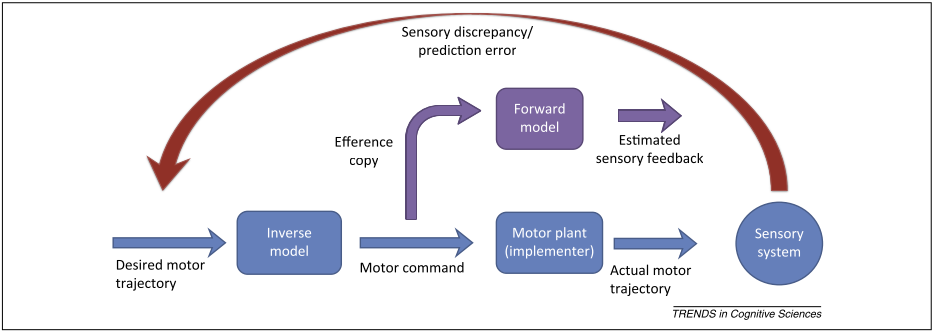
\includegraphics[scale=.3]{images/AFM.png}
      \caption{The Auxiliary Forward Model of motor control}
        \label{fig:AFM}
   \end{center}
\end{figure}

\begin{figure}[htbp]
  \begin{center}
    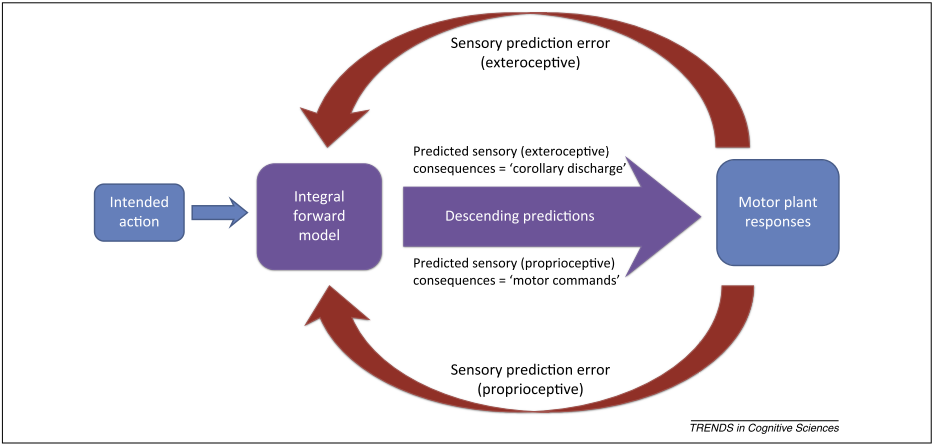
\includegraphics[scale=.3]{images/IFM.png}
      \caption{The Integrated Forward Model of motor control}
        \label{fig:IFM}
   \end{center}
\end{figure}


Both the AFM and IFM approaches agree that prediction, error minimisation, and hierarchical modelling are core processes in human cognition. From a thermodynamic standpoint, however, IFM appears to offer a more efficient model for free energy minimisation.  By replacing motor commands with direct predictions about proprioceptive and exteroceptive consequences, the need for a distinct optimal control calculation (i.e. an inverse model) disappears and along with it the need for an efference copy of the motor command, thus implicitly minimising various energetic costs \citep{Pickering2014,Friston2010}.   In place of the auxiliary mechanisms of the AFM, IFM posit a more complex (distributed) forward model mapping prior beliefs about desired trajectories to sensory consequences.  Whereas the ``heavy lifting'' in AFM required the use of an efference copy and inverse models, in IFM this work is done by the acquisition and use of a more complex predictive (generative) model \citep{Pickering2014}.


EXPLAIN: with reference to TICKLING?



%According to the AFM account, the forward model is distinct from the inverse model, because it involves apparatus that computes the motor commands used to drive online action. Such a model is thus free to depart considerably in form from whatever governs the true kinematics of the agent.  Furthermore (in AFMs) the outputs of the forward model (i.e., the corollary discharge) do not cause movements – they are just used to finesse and predict outcomes and in learning.

%Comparisons between downward sweeps of prediction and upward sweeps of sensory input lead to a cascade of error signals throughout the hierarchy. These error signals are used to adjust the forward models that are guiding action execution (Clark, 2013). Importantly, actions are aimed at minimizing prediction errors, by matching sensory inputs to predictions— a process termed active inference (Friston, 2008;Friston & Frith, 2015a, b). Eventually, active inference leads iteratively to a solution that will take the organism from its current motor state to the desired one.



\subsubsection{Predictive Coding and Predictive Processing}
Research suggests that models capable of maintaining organismic regulation with the environment (i.e. by reducing free energy) must be able to anticipate sensory inputs before they occur. As Pickering and Clark explain, ``predictions can power learning, help finesse time delays, and enable a suite of potent capacities for motor imagination and simulation-based reasoning'' \citep[6]{Pickering2014}.  The ``predictive coding'' hypothesis depicts a brain that is constantly in the (tricky) business of anticipating probable worldly sources of sensory signals, and adjusting action schemas in order to minimise the error of these predictions (or maximise the precision of these models) \citep{Friston2010,Clark2013}. Predictive coding offers neurocomputational architecture for the thermodynamic approach to cognition.

Data compression strategy:

Neurocomputational evidence suggests that predictive coding is supported in the brain by multilevel and hierarchical arrangement of cortical structures, which enable bi-directional cascades of information between levels.  Higher levels of the cortical hierarchy formulate models based on prior experience, which are employed to ``explain away'' sensory signals at lower levels. Lower level signals unaccounted for by higher level predictions are incorporated into higher level structures and strengthen the robustness of the model.  Predictive coding has been likened to a process of ``empirical Bayes,'' whereby prediction errors function to strengthen prior probability distributions of models for future inference \citep{Robbins1964}, and representations of uncertainty around sensory signals are factored into the predictive model itself \citep{Clark2013}.  The brain's capacity to quantify the uncertainty of any given sensory state facilitates optimal selection between competing predictions pertaining to the same bottom-up sensory signals, judged probabilistically.  At any one moment, an individual has access to multiple hypotheses derived from priors, which compete for the best fit of the sensation, until that process leads to fixation on the best hypothesis for the sensory state.
Binocular rivalry, (for example looking at a necker cube) is an instance in which there is insufficient sensory information available in order to reach fixation on one model over another (see Image ~\ref{fig:neckerCube} \citep{Frith2007}.

\begin{figure}[htbp]
  \begin{center}
    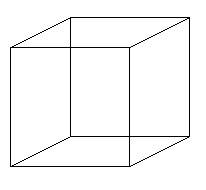
\includegraphics[scale=.7]{images/Necker_cube.png}
      \caption{Necker Cube: The binocular rivalry is associated with insufficient sensory information}
        \label{fig:neckerCube}
   \end{center}
\end{figure}


\subsubsection{Active Inference}

Importantly, in the case of motor systems, agents are able to move their sensors in ways that amount to actively seeking or generating the sensory consequences that they (or rather, their predictive models) expect.  In this way, ``error signals self-suppress, not through neuronally mediated effects, but by eliciting movements that change bottom-up proprioceptive and sensory input''  \citep[][1349]{Friston2003}.  This form of ``active inference'' involves the functional and temporal integration of perception, representation, and action to fulfil an ever evolving set of sub-personal expectations about the state of the world.  Perception, cognition, and action work closely together to minimise sensory prediction errors by selectively sampling, and actively sculpting, the stimulus array.


The Outfielder's Problem:


The combination of predictive coding and active inference provide the theoretical machinery necessary for a thermodynamic understanding of cognition.  The result is a welcomed conceptual shift away from individual-centred computational models of information processing (originally inspired by the mechanics of the electronic computer), which tend to render cognition as the final product of a linear sequence of sensory perception, amodal mental representation, and action selection \citep{Lewis2005}.  By contrast, thermodynamic cognition offers a model in which perception, representation, emotion, and action are functionally and temporally integrated in the service of informational processes of free energy minimisation.  Importantly,  to conceive of social cognition in this way, as an embodied, embedded, and immediate process of inference, centralises the role of automatic movement regulation strategies---traditionally classed as ``lower-cognitive'' processes---in establishing and maintaining the transfer of information between individuals, within groups, and throughout populations---traditionally thought to be executed by  ``higher-cognitive'' processes \citep{Claidiere2014}.
In the following section I outline the degrees of freedom problem associated with human movement, and explain how humans have devised novel cognitive solutions to it.  Many of these solutions can be observed in joint action scenarios.


\subsubsection{The degrees of freedom problem and its solutions in human movement}

Bernstein \textcite{Bernstein1967} was the first to point out the astounding computational challenge associated with coordinated physical movement in multi-component living systems.  In the case of human intra-personal movement, for example, an impressive balance is somehow struct between flexibility, precision, and control, whereby hundreds of muscles and joints coordinate to perform many different tasks of everyday life.  When we grasp a cup or catch a ball, many individual muscles and joints---each with their degrees of freedom---work together in fine concert.  Bernstein found it unlikely, from a computational perspective, that the central nervous system would be able to finely control all the possible movements (the degrees of freedom) of each single muscle individually to create coherently directed movements---it would be computationally impossible. Rather, he suggested that muscles and joints form  ``functional synergies''---flexible function-specific self-organising assemblies---by locally coupling and constraining each other’s degrees of freedom to greatly reduce the amount of control needed.

Functional synergies are higher-order control systems formed by coupling movement system degrees of freedom \citep{Turvey1978}.  Functional synergies are defined by two core properties:  1) dimensional compression (potentially independent DF are coupled so that the synergy possesses a lower dimensionality than the set of components from which it arises) and 2) reciprocal compensation (the ability of one component of a synergy to react to changes in others).
The existence of functional synergies have been identified on multiple levels of behaviour, from brain function \citep{Yufik1998,Sengupta2013}, to interpersonal interactions \citep{Kelso2009,Riley2011,Fusaroli2014}, to large-scale human societal dynamics \citep{Nowak2017}.  It is currently understood that functional synergies in human movement systems are regulated by a continuum of processes that span interoceptive action-orientated predictive models on one end, to  basal (lower-cognitive) movement regulation mechanisms that enable direct (i.e., largely extra-neural) coupling with the task-specific environment \citep{Semin2012}, on the other.  Across this continuum, the priorities of thermodynamic cognition remain consistent: free energy is minimised, either by more precise and flexible (but cognitively expensive and slow) predictive models on one end of the continuum, or by more automatic and situated processes that outsource cognitive demands to affordances of the task environment, on the other end of the continuum.

%Interoceptive feedback underlies the feeling of grasp, or understanding that accompanies the organization of disparate “representations” into cohesive structures amenable to further operations (mental modelling).

Intra-personal and interpersonal human movement both rely on the nervous system’s capacity to anticipate, attend, and adapt to the conditions of the environment \citep{Keller2014}.  In the case of intra-personal human movement, successful coordination of is made possible by direct and habituated coupling of movement control system to the organism's various degrees of freedom.  Predictive models for interpersonal movement, for example, appear to benefit from more privileged access to exteroceptive and proprioceptive feedback than predictive models generated to account for the movements of others.  By contrast, interpersonal movement coordination poses a much more significant challenge.  In the case of interpersonal coordination, the combination of 1) limited reliability of sensory modalities as a source of information about the action of others \citep{Wilson2005,Wolpert2003,Frith2007} and 2) the informational complexity associated with a cognitive system comprising multiple autonomous agents \citep{Bernstein1967} means that successful coordination in joint action is an inherently difficult and highly improbable cognitive challenge.

\subsection{Solutions to the problem of joint action}

Vesper textcite{Vesper2010} outlines a minimal architecture for joint action, which contains three components:

\begin{enumerate}
  \item Represent a shared goal, as well as representing one’s own individual contribution to the shared goal.
  \item Apply monitoring and prediction processes to each partner’s actions. This includes monitoring the extent to which shared goals or tasks are being fulfilled while at the same time predicting a partner’s actions.
  \item Facilitate continuous coordination via coordination smoothing, defined as the process of continuously improving one’s prediction of the partner’s action.
\end{enumerate}

It is unlikely that solutions to these minimal requirements of joint action could be driven solely by central, executive control processes in the central nervous system---joint action would be too slow and costly. It is similarly unlikely that processes of unconstrained automatic alignment with no higher-level coordination could possibly enable joint action---joint action would be too undirected and chaotic \citep{Fusaroli2014}.  Rather, it seems more plausible that joint action is facilitated by a continuum of mechanisms spanning executive control through to direct coupling.  To establish and sustain interpersonal coordination, participants selectively recruit multiple behaviours and processes, which in turn become more interdependent and constrained by the function of the ongoing activity.

Current research suggests that faculties for joint action involve re-purposing of mechanisms core to successful intra-personal coordination, such as 1) predictive action-orientated models \citep{Vesper2012}, direct coupling of action and perception networks \citep{Novembre2014}, and lower cognitive mechanisms of movement regulation \citep{Semin2008,Riley2011}.  Generally speaking, these solutions appear to exist on a continuum, with more (neuro)computationally intensive mechanisms of anticipation, attention, and adaption occupying one end, and more direct (i.e. extra-neural) coupling with external components of the movement system, occupying the other end.  Successful joint action relies on the recruitment of a suite of mechanisms from this continuum in order to establish and sustain interpersonal coordination.  Evidence discussed below suggests that optimal solutions to joint action may tend to recruit more extra-neural resources to minimise free energy, whereas less efficient solutions to joint action may rely on more computationally intensive procedures in order to reduce free energy.

In the sections below I will review evidence for a continuum of solutions in joint action, grouped under 1) interoceptive predictive models 2) action-perception links and 3) direct extra-neural coupling.


\subsubsection{Interoceptive predictive models}
Current research in joint action suggest that interoceptive predictive processes are at the core of successful human social interactions \citep{Graziano2013,Manera2013,Sparenberg2012,Springer2012}.  The essence of this proposal is that we use our own cognitive resources to build mental models of other people’s cognitions and the shared tasks that we share with others \citep{Tomasello2005a}.  Simulation of other people’s cognitive states (e.g., what they are feeling, thinking, and attending, a.k.a. a theory of mind) guide our expectations about their future behaviour, and in this way contribute to the viability of social interactions.

Recently, both AFM and IFM approaches have been applied to joint action research.  Keller and colleagues (2016), for example, presented a conceptual framework that applies AFM approach to musical joint actions.  The authors suggest that ensemble music making, such as a string quartet, requires three types of internal models:
1) self-internal models responsible for action planning and motor control, 2) other-internal models that support the prediction of other’s actions, and 3) joint-internal models, which keep a dynamic representation of the shared goal \citep{Keller2016}.  Among these three types of models, only self-internal models comprise inverse models that output motor commands and efference copies of one’s own actions as forward models.  Each member of the quartet has different self-internal models of the notes played by their own instrument, and will have expectations about the notes that they hear from other instruments and the overall sound of the joint performance.  ``Compensatory control'' (the ability to correct deviations from the shared goal) is achieved by updating self-inverse models using the error signal obtained from comparing the actual joint state and the joint desired state; ``anticipatory control'' (the ability to execute actions based on predictions) is achieved by an adaptation signal that results from the comparison between predicted joint state and the desired joint state.
E:

Pesquita and colleagues (2017) identify three shortcomings of this application of AFM to joint action.  First, the AFM approach does not explain how prediction error feedback reaches the model of the shared goal.  This issue limits the model’s ability to account for flexible joint goals in joint action (e.g., switching between the shared goal of carrying a table or the bench depending on the location of both objects).  Second, the AFM approach lacks an mechanism that allows sensory feedback to reach the other-internal model. In the present model, predictive joint-error signals are fed-back only to the self-inverse model, and no inverse model for the joint action partner exists. This missing link suggests the practical possibility that self and other models may gradually diverge over time \citep{Pickering2014}.  Third, Keller et al.’s proposal does not specify how sensory input is differentially used to update self and other models, which limits the model's ability to account for learning and adaptation within joint action \citep{Pesquita2017}.  Thus, not only does the AFM approach appear to be computationally intensive due to the recruitment of auxiliary inverse models and dual motor commands (explained above), it also appears to be unable to fully account for the completeness and flexibility of real-world joint action.

As Wolpert himself points out, movement is a complex process, because there are often several solutions that may lead to the desired outcome, the information available for selection is often distorted and delayed (due to neural-muscular limitations), and the external environment is dynamic \citep{Wolpert1997}. Without an obvious solution to the shortcomings mentioned above, it is difficult to apply the AFM approach concretely to a large number of real-world social interactions where actors do not subscribe to the same interaction end-goal, which is often instead open-ended and multifaceted \citep{Pesquita2017}.

\myparagraph{Predictive Joint Action Model}
In place of the AFM approach, Pesquita and colleagues \textcite{Pesquita2017} propose an IFM approach that accounts for the minimal requirements of joint action.  The model, which they call a ``Predictive Joint Action Model'' (PJAM), is comprised of three hierarchical levels of inference: goal representation, action-planning, and sensory routing (see figure ~\ref{fig:PJAM}). PJAM assumes that each participant in a joint-action maintains internal models of 1) the joint task, 2) the action contributions of self and others to the joint task, and  3) the sensory-motor inputs expected from action plans.  In line with the IFM approach, PJAM does away with auxiliary processes of motor control and efference copies, and posits instead that joint action emerges directly from two or more individuals converging on equivalent predictive models for joint action.

\begin{figure}[htbp]
  \begin{center}
    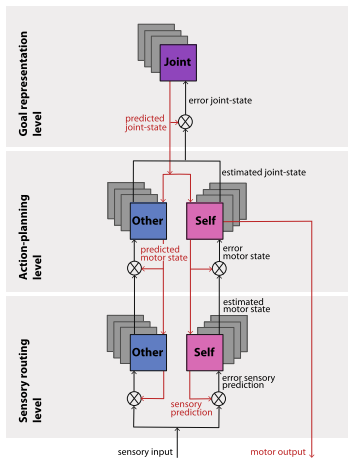
\includegraphics[scale=.8]{images/PJAM.png}
      \caption{The Predictive Joint Action Model \citep{Pesquita2017}}
        \label{fig:PJAM}
   \end{center}
\end{figure}

The goal-representation level of PJAM suggests that participants in joint action generate and monitor representations of the shared task. This proposal is formulated from evidence that musicians maintain shared representation of desired unified sound of an ensemble \citep{Keller2008}.  In one study, for example, Loehr and colleagues  use a neurophysiological measurement that codes unexpected events (ERP) to show that musicians tracked deviations from a desired joint state \citep{Loehr2013}; in another study, Loehr and Vesper \textcite{Loehr2016} demonstrated that playing music together generates shared expectations regarding the desired state of joint action, and this process guides future action.  Taken together, this evidence suggests that participants in joint action utilise prediction errors arising from lower levels to update representations of shared tasks.
%(Wolpert MOSAIC model doesn't account for updating rep. of shared task)

At the action-planning level of PJAM, pairs of models represent the expected contributions to a joint-action of self and others.  This level of the model is supported by evidence that participants in joint action generate internal models of self and other, known as co-representation, either spontaneously and involuntarily, as in the commonly used social simon task experimental paradigm \citep{Sebanz2003,Atmaca2008}, or more deliberately, as in a coordinated dyadic horizontal jumping task \citep{Vesper2012}.  Studies show that co-representation is modulated by mood \citep[positive or negative affect, see][]{Kuhbandner2010}, self-concept and social orientation \citep{Colzato2012,Colzato2012a}, and group membership \citep{DeBruijn2008,Iani2013}.

Action-planning entails, on the highest level, action roles (); on a mid-level, movement trajectories (); and on the lowest level, movement of muscle groups of self and others.  As with goal representation, action-planning for self and others is a predictive process \citep{Flanagan2003}, in which individuals encode motor predictions and resulting errors of others' actions in addition to their own \citep{VanSchie2004,Radke2011}.  Predictive models of self and other action plans appear to be grounded in an individual's own motor simulation processes, such that each participant maintains covert motor activations relating to expected contributions of their partners \citep{Hollander2012}.  There is evidence to suggest that motor simulation of self and other action plans is mediated by the existence of a shared goal between co-actors \citep{Kourtis2010}.  Loehr and Vesper \textcite{Loehr2016} demonstrate that when learning a joint piano piece, musicians are able to better perform the piece together rather than solo, which suggests that representations about each participant in joint action are encoded within the joint context of the interaction.  In other words, when we learn a joint task we not only learn our own role, but also the impact of other's roles on our own role in the joint action.  In sum, the action planning level of PJAM proposes that models of the self and models of partners can be paired to represent the possible combinations of individual contributions to the joint action. These models transform the desired joint-state signal, descending from the goal representation level, into expectations of the unique motor states of the self and the partner.  Error signals arrive from levels of the model below, with sensory routing.

The sensory routing level receives the inflow of sensory input and compares it to internal model predictions pertaining to each participant's action outcomes.  This comparison process serves as a gate for parsing sensory information into their corresponding predictive streams (self or others, see Figure ~\ref{fig:PJAM}), which allows the predictive system to attribute external consequences to each individual’s actions.   For example, two people carrying a table will receive haptic input from the table. This input will be confounded with respect to its source, in that the haptic input itself does not differentiate between the forces that each brother applies to the table. However, the comparison between the haptic input and the separate predictions about one’s own and the other’s action will help feed each predictive cascade of self and other into their respective streams \citep{Pesquita2017}.

Consistent with other levels of PJAM, deviations between sensory input and sensory predictions (i.e., sensory predictive errors) are fed-back to sensory predictive models in order to continuously improve sensory parsing.  Evidence indicates that accurate predictions of others actions is associated with the dampening of the sensorial experience of joint action outcomes.  Predictions about motor outcomes are used to filter out the sensory feedback produced by the same action \citep{Blakemore1999}.  This proposal is confirmed by evidence that greater sensorial experience occurs when an outcome is unexpected, as oposed to predicted from prior self or other action \citep{Sato2008}.  In addition, attributing sensory consequences to joint action partners is linked to cooperative success \citep{Chaminade2012}, suggesting that finely tuned sensory routing based on predictions of self and other actions could be key to successful coordination.

PJAM is inspired by proposals made by Friston and Frith (2015, 2015a) \citep{Friston2015,Friston2015a}, who build upon theories of active inference and predictive processing to suggest that joint action entails two (or more) brains committed to modelling each other in order to minimise free energy.  In this scenario, when coordinating in joint action, brain A has a model of brain B, which in turn has a model of brain A, and so on---\textit{ad infinitum}.  The recurrent predictions of both brains about one another threatens an infinite runaway regress that could preclude accurate modelling of either brain.  As Frsiton and Frith show, however, this recursion mathematically dissolves if the models of the two brains are formally similar \citep{Friston2015}.  Grounded by their computational similarity derived from a shared narrative, each brain is able to generate predictions of the sensory outcomes caused by itself and the other in the same way.  The authors propose that this will lead to generalised synchronisation between the internal models of both brains, such that they will be able to accurately predict each other's behaviour based on feedback of exteroceptive (sensory information from the deriving from the actions of others and the task environment) and proprioceptive (pertaining one's own contribution to joint action) prediction errors.

In real world joint action scenarios such as interaction team sport, co-actors interact and rehearse their behaviours to produce a hierarchy of aligned representations, an implicit common ground on which joint action can unfold \citep{Noy2017}.  PJAM provides a framework for the function of interoceptive predictive modelling in these processes of alignment.  Each level of PJAM generates predictions of the information that it expects to be found on the level below.  Continuous comparison between adjacent levels results in error signals that are sent up to optimise subsequent predictions in the level above.  This hierarchical predictive architecture for joint action allows humans to generate accurate yet flexible models for joint action. The combination of accuracy and flexibility comes at a cost, however, and it is clear that humans also utilise, in addition to interoceptive modelling techniques, a range of more direct and extra-cortical mechanisms in order to establish and maintain joint action with others.


\subsubsection{Action-perception links}

Alongside research into predictive processing and interoceptive action-oriented modelling in the brain, research in psychology \citep{Prinz1990,Prinz1997,Prinz2013}, neurophysiology \citep{Rizzolatti2004,Rizzolatti2010}, and neurocognition \citep{Wolpert1998,Wolpert2000} has produced compelling evidence that interpersonal behavioural coordination in joint action could be further facilitated by the intrinsic coupling—--under certain circumstances---of action perception and action execution in the human brain.  Since Prinz’s (1990) initial proposal that perception and action are coded in a common representational domain, and are therefore linked by shared neural resources, research into action-perception coupling has spanned individual action as well as interpersonal social interaction.
In terms of its function for joint action scenarios, action-perception coupling is regarded as a basic link between sender and receiver \citep{Rizzolatti1998} that provides procedural, perceptual, and emotional common ground between individuals \citep{Sebanz2006}

In essence, action-perception coupling refers to the ostensive co-occurrence of a stimulus for action and its motor representation.  For example, the representation of a perceptual effect (say the sound of a middle-C on a piano) can trigger the movement necessary to produce the effect itself (motor instructions for playing the middle-C key on a piano).   Importantly, evidence suggests that sensory-motor coupling emerges primarily as a result of motor learning: having only visual \citep{Candidi2014} or auditory \citep{Lahav2007} experience with a given action is not sufficient to trigger these motor responses—active motor learning is necessary.  As such, most research into action-perception coupling occurs with individuals who have mastered a certain sensorimotor task, such as expert musicians, whose movements and intended sounds become strongly associated \citep{Novembre2014}.

In behavioural experiments in which samples of musicians are compared to non-musician controls, researchers demonstrate that auditory perception primes action if strong action-perception links have been established through instrument-specific training \citep{Drost2005,Drost2005a,Drost2007}.  For example, Drost and colleagues showed that sound cues incongruent with the prescribed action response (the sound cue of a D chord when the prescribed action response is a C chord) delayed execution time \citep{Drost2005} and induced more false responses \citep[i.e., production of the heard chord, instead of the imperative one,][]{Drost2005a} in pianists but not non-pianists.  Keller and Koch \textcite{Keller2006} showed that mental images of anticipated action effects can prime responses to a similar degree as is observed with congruent and incongruent sounds, highlighting the role of action-perception coupling in action preplanning (i.e., before sounds are actually perceived).  Further studies demonstrated that action-perception coupling does not only enhance the efficiency of action planning, but also facilitates timing accuracy and economical force control by optimising movement kinematics \citep{Keller2010}.

Neurophysiological evidence suggests a neural signature for action-perception coupling in the motor cortices.  Haueisen and Knosche \citep{Haueisen2001} conducted a magnetoencephalography (MEG) study (piano players with and without experience) and showed that perception of piano pieces led to an increase of neural activity over the motor cortex hand area in piano players but not non-musicians.  Bangert and colleagues \textcite{Bangert2006} ran an fMRI study where professional pianists and non-musicians heard novel piano sequences that were synthesised online (and therefore could not be familiar).  Compared to non-musicians, professional pianists showed a broad network of motor areas responding to the piano sequences, including both primary motor and premotor (BA 4/6) regions.  Besides auditory- and visual-motor coupling, tactile, proprioceptive and haptic sensory feedback has been shown to induce coupling \citep{Schulz2003,Kuchenbuch2014}.

These behavioural and neurophysiological data, taken together, indicate that musical training leads to the emergence of cross-modal action-perception coupling, where perception of the effects of musical actions (either the sounds produced or the visual presentation of the movement patterns) triggers a representation of the movements necessary to produce these effects. Interestingly, these effects have also been observed in trained non-experts \citep{Bangert2003,Lahav2007}.  Lahav and colleagues (2007), for example, trained non-musicians to play a piano piece by ear (without notation) over a period of five days and found that activation of the frontoparietal motor-related network (comprising Broca’s area, the premotor region, the intraparietal sulcus, and the inferior parietal region) increased most strongly for the trained pieces, versus untrained (but motorically known) and familiar but motorically unknown pieces.

It has been argued that the function of action perception coupling is twofold.  First, coupling of this nature supports a neurophysiological capacity to anticipate (generate predictions about) our own as well as other's  (i.e., observed) actions.  Maidhof et al. \textcite{Maidhof2009} and Ruiz et al. \textcite{Ruiz2009} conducted two similar EEG studies in which they examined the ERPs preceding the execution of piano errors in pianists and non-musicians.  In pianists (but not non-musicians) errors were detected prior to their execution (the EEG signal was found to anticipate the actual mistake by 100 ms \citep{Maidhof2009} and 50–70 ms \citep{Ruiz009}.  These data thus indicate that the coupling of sensory and motor cortices has a strong anticipatory character that, given the existence of an association between movements and their ensuing effects, permits the generation of predictions about the state of our own body and the sensory consequences of our movements.

Second, action-perception links act as a resource for the co-representation of and coordination with others in joint action.
Research demonstrates that the training-mediated coupling of perception and action is not confined to individual behaviour.  As mentioned above, there is evidence to suggest that expert ensemble musicians form representations of self and other-related actions, and that these representations are influenced by properties of the individual’s own motor system \citep{Novembre2012}.  Action-perception links can be used for monitoring and integrating (e.g., timing or combined pitches) the actions of other ensemble members with self-generated actions \citep{Loehr2013}, and these effects appear to be stronger in individuals with high perspective taking skills \citep{Novembre2012,Loehr2013}.  The overlap between mechanisms for action production and action observation suggests that individuals may represent their own and others’ actions in a commensurable format.  Training-induced motoric representation of self and other actions may facilitate various capacities important for joint action, such as prediction, adaptation, and entrainment.


\subsubsection{Extra-neural direct coupling}
There is also evidence of extra-neural solutions to the problem of high cognitive uncertainty joint action problems. Establishing and sustaining direct coupling with resources of the joint action environment, namely other actors and the physical resources of the task-specific environment, can help solve Bernstein's degrees of freedom problem.   In interactive, cooperative tasks, individuals have been found to couple and reciprocally constrain their movements reducing the overall control needed to maintain effective cooperation \citep{Ramenzoni2011,Ramenzoni2012,Riley2011,Schmidt1990}.  Individuals’ behaviours become increasingly interdependent, so that a higher-level structure of the interaction emerges. This kind of emerging organisation has previously been referred to as soft-assembly \citep{Kello2009}: individuals preserve a degree of autonomy, but their behaviour is constrained by the interaction. They can flexibly engage and disengage from it, as well as become part of other soft-assemblies \citep{DeJaegher2010,DiPaolo2012}.

Research into the coordination dynamics of natural joint actions  has shown evidence of dynamic coupling (synchronisation) in joint-action tasks, such as dancing, martial arts, and moving objects like furniture.  In these studies, specific component degrees of freedom are modelled as coupled oscillators (using the HKB model \citep{Haken1985,Kelso1986}, which describes the change in the relative phase between two oscillatory components).  Models are analysed for non-random fluctuations in relative phase over multiple time scales.  This type of synchronisation is said to be of a fractal or semi-fractal organisation, also known as 1/f scaling or ``pink noise'' \citep{Caron2017}. According to Anderson and colleagues \citep{Anderson2012}, 1⁄f scaling is ubiquitous in smooth cognitive activity, and indicates a self-similar structure in the fluctuations that occur over time (within a time series of measurements).
1⁄f scaling indicates that the connections among the cognitive system's components are highly nonlinear \citep{Ding2002,Holden2013,Kello2010,Riley2011,VanOrden2003,VanOrden2005}. Pink noise has been measured beyond dyadic synchronisation, in the analysis of sub-phases of team sports \citep{Passos2014,Duarte2012} and group dancing \citep{Chauvigne2017}.\footnote{1⁄f scaling is temporal long-range dependencies in the fluctuations of a repeatedly measured behaviour or activity. Analogous to spatial fractals, 1⁄f scaling denotes a fractal or self-similar structure in the fluctuations that occur over time. That is, higher frequency, lower amplitude fluctuations are nested within lower frequency, higher amplitude fluctuations as one moves from finer to courser grains of analysis \cites(for a more detailed description see, for example)(){Holden2005}{Kello2009}}

In addition to the pink noise of dynamic coupling in joint action, research has also attempted to capture movement signatures of joint action that can capture the phenomenon of ``group flow'' \citep{Sawyer2006} or being ``in the zone.''  Working within the common dyadic ``mirror game'' paradigm, for example, Noy and colleagues \textcite{Noy2011,Noy2015,Hart2014} have developed an experimental proxy for an optimal state of togetherness in joint action.  ``Co-confident motion'' (CC motion) is canonical movement pattern of synchronised motion characterised by smooth and jitter-less motion, without the typical jitter resulting from reactive control in more commonly encountered leader-follower patterns.  In CC motion, different players appear to shift their basic motion signatures to a movement shape that is altogether different from their individually preferred shapes \citep{Hart2014}. Importantly, the pattern of CC motion shares the same sine wave shape as the optimal solution of the minimum jerk model, a well-known motor control model for rhythmic motion \citep{Hogan2007}. Noy and colleagues suggest that it is possible that during CC motion periods of joint action, two players converge to a canonical pattern stemming from an optimal state of each participant’s motor control system.  The resulting motion may be easier to predict and to agree on. Furthermore, participants appear to use smooth elementary strokes of CC motion as the building blocks for more complex motion \citep{Noy2017}.  This observation raises the possibility that CC motion, a state of alignment in which individual components converge in a transcendent, functional synergy, could set the cognitive foundation for more efficient and effective higher level processes of communication and information transfer \citep[15]{Lerique2016}.

  % Experimental evidence has shown that functional interpersonal synergies facilitate performance of social cognitive or linguistic tasks, such as gaze coordination and turn taking in conversation \citep{Miles2010,Richardson2005,Shockley2009}.  Conversely, being psychologically distanced from another individual can inhibit the emergence of interpersonal synergies \citep{Miles2010}.  The ways in which functional interpersonal synergies facilitate adaptive information transfer between individuals and within groups suggests that psychological mechanisms and cultural practices responsible for generating these synergies could have been subject to cultural evolutionary forces of selection and attraction \citep{Claidiere2014,Mesoudi2016a}.

  \subsubsection{Individual differences}


  Research suggests that preexisting dispositional tendencies in sociality dimensions of personality (e.g. extroversion, agreeableness) and social orientation (locus of control, communication styles), as well as the nature of pre-existing interpersonal relationships, and technical competence in joint action \citep{Novembre2014}, will impact on the structure and quality of interpersonal movement coordination and, presumably, the social unity that emerges from joint action \citep{Marsh2009}.

  The personality concept of empathy—understanding others’ thoughts and feelings—has been linked to anticipatory mechanisms related to action simulation \citep{Sevdalis2014,Keller2014}.  In the piano studies mentioned above \citep{Novembre2012}, scores on the ‘perspective-taking’ sub- scale of an empathy questionnaire correlated positively with neurophysiological measures of representing the other’s part in their own motor system, as well as how much this ‘other-representation’ was relied upon for coordination \citep{Novembre2014a}.
  in a synchronized finger-tapping task, Pecenka and Keller (2011) found that scores on a perspective-taking questionnaire correlated with the degree that individuals predicted event micro-timing in a tempo-changing pacing sequence.  Richardson and colleagues (2007) found in a dyadic plank moving experiment, individuals’ levels of agreeableness and extroversion were positively correlated with persistence of cooperation in the task.

  Social orientation and motivation have also been shown to effect interpersonal coordination.  A study of unintentional coordination revealed that prosocial-oriented individuals spontaneously synchronised arm movements with others more than pro-self-oriented individuals, whether their social/self-orientation reflected their pre-existing disposition or resulted from an experimental manipulation \citep{Lumsden2012}.  Studies have found that interacting with a late-arriving partner reduced stepping synchronisation, compared with interacting with a partner who arrived on time \citep{Miles2010}, and bodily synchrony decreased during arguments compared with affiliative conversations Paxton2013.

  A recent study addressed the relationship between locus of control (i.e. the degree to which life events are perceived to result from one’s own actions) and temporal adaptation (error correction) \citep{Fairhurst2014}.   Results indicated that individuals with an internal locus of control (who attribute the cause of events to their own actions) engaged in less phase correction than individuals with an external locus of control (who attribute events to external factors), which may reflect individual variation in predispositions towards different movement coordination strategies.  This assertion is corroborated by a study conducted by Schmidt and colleagues \textcite{Schmidt1994}, which used interpersonal wrist-pendulum coordination to investigate the effects of self-reported social competence \citep{Riggio1996} upon social coordination stability.  Subjects were selected to create homogeneous social competence dyads (High–High or Low–Low pairs) and heterogeneous dyads (High–Low pairs). The heterogeneous (High–Low) pairs demonstrated significantly greater stability and fewer breakdowns in coordination than the homogeneous (High–High and Low–Low) social competence pairings, suggesting that reciprocity (leader-follower) rather than symmetry (leader-leader or follower-follower) of social competence facilitates social coordination.  In this sense,  ‘internal’ individuals may stabilise the tempo of their own performance (at the expense of synchrony) and take a leader role, whereas ‘external’ individuals may synchronise with their partner (at the expense of maintaining a steady tempo) and take a follower role.  In sum,  dispositional tendencies movement coordination and in sociality dimensions might set the initial conditions that make pull to the cooperation attractor stronger (or weaker) than a pull to the autonomy attractor (independent action).


\subsubsection{Culture}

Joint actions that involve complex sequences and divisions of labour between participants appear to rely heavily on capacities to explicitly signal intention for the assigning of roles, forward planning, and repair of failed coordination \citep{Frith2010}.  These ``coordination smoothers'' \citep{Vesper2017} often function to reduce spatial and temporal variation in action by providing a shared spatiotemporal referent for co-alignment of predictions.  Cultural conventions are examples of effective framing devices for joint action.  Depending on the context of the joint action, it could be subject to a pre-existing, mutually recognised power relations typical in the established culture (e.g., favouring hierarchical or egalitarian communication, \citep[see]{Cheon2011}) and the particular situational context (e.g., formal or informal).
Establishing roles, such as leader or follower, also has a similar smoothing effect, and often the affordances in the task environment shape the smoothing strategies available to co-actors \citep{Marsh2009}.

A key insight overlooked by the existing social high account of group exercise and social cohesion, but revealed by the paradigm shift surrounding the social cognition of joint action, is the sensitivity of joint action (or any cognitive process for that matter) to informational affordances provided by various layers of ecological and cultural context.  The cognitive inputs to joint action in real world settings are rarely limited to essentialised components administered in laboratory paradigms. It is known that cognitive processes relevant to joint action are distributed throughout brains, bodies, and the physical environment of the ecological niche in which it is situated.  There is evidence to suggest that joint action co-participants rely on a series ``frames of reference'' for joint action execution \citep{Ray2018}, and it appears that social interaction functions best in situations where there is a snug fit between individuals' implicit cultural expectations and explicit rules for engagement \citep{Vollan2017}.

Shared cultural knowledge can act as a ``coordination smoother'' \citep{Vesper2017} for joint action, enhancing the effectiveness and efficiency of joint action between co-participants who share a similar informational framework.  In the predictive processing paradigm, cultural habits and frames of reference can be seen to act as ``hyper-priors'' that set the macro-contextual coordinates for joint action\citep{Clark2013}.  According to the PJAM framework, affordances for joint action are dictated by processes operating at multiple hierarchical levels---from the micro-level predictive processes associated with movement action and perception, to the macro-level predictive frames offered by specific cultural and contextual niches---interact in complex processes of reciprocal causation to shape joint action.


%Conceptualisation of the causal complexity of cognitive processes relevant to joint action in this way echoes a broader reconceptualisation of the causal complexity associated with change on an evolutionary timescale, which recognises that human behavioural phenomena is the result of a number of biological, cognitive, and ecological mechanisms that interact via reciprocal feedback loops spanning varying scales of time and space \citep{Fuentes2015}.

  %The experimental approach to science requires re-evaluation in light of an emerging paradigm emphasising distribution of cognitive processes throughout an array of coordinated informational affordances.


\subsection{More efficient joint action relies on more on direct coupling?}

The thermodynamic mandate of free energy minimisation predicts a tendency towards more efficient solutions to the challenges of joint action, without compromising task-specific function.  While interoceptive predictive models are flexible and effective for the purposes of establishing and maintaining coordination in joint action, they do come at a (computational) cost.  The thermodynamic approach to joint action predicts that more efficient and effective joint action will recruit mechanisms and strategies that outsource the computational cost of joint action to sources beyond the brain. In the case of highly skilled practitioners, whose interoceptive predictive models are presumably highly attuned to the affordances of the task environment, it is plausible that extra-neural and even extra-personal resources could provide a more cognitively efficient and effective route to the performance of successful joint action.  In which case, it is possible that the tacit and sub-perceptual quality of ``team click'' in joint action could be indirect phenomenological evidence of optimal movement coordination.

Interestingly, studies of highly skilled practitioners in joint action demonstrate that more technically competent practitioners generate more accurate predictive models for joint action than less technically competent practitioners \citep{Tomeo2012,Aglioti2008,Mulligan2016}.   In studies involving skilled versus non-skilled practitioners in dyadic interactions, it has been shown that more skilled practitioners create stronger dynamical coupling through flexibly modulating their actions with others \citep{Schmidt2011, Caron2017}. These findings are corroborated by other studies that find that professional footballers (versus novice controls) are able to more accurately predict the direction of a kick from another player's body kinematics (\cite{Tomeo2012}, see also \cite{Aglioti2008,Mulligan2016} for similar results with basketball and dart players).

Interestingly, when analysing co-regulation between members of basketball teams, it was shown by Bourbousson \textcite{Bourbousson2015} that more expert teams made fewer mutual adjustments (at the level of the activity that was meaningful for co-actors), suggesting an enhanced capability of expert social systems to achieve and maintain an optimal level of awareness during the unfolding activity, potentially implicating down-regulation of prediction error management processes, and greater reliance on extra-neural couplings with co-actors and the physical environment.

A recent field study by R'Kiouak and colleagues (2016) supported this line of reasoning.  Through combined analysis of phenomenological and video data derived from a close study of two unacquainted expert rowers who participated in a real world dyadic rowing exercise (coxless pair), the authors found that athletes reported joint action as being salient and meaningful only 24.5\% of the race under study (e.g., during synchronisation breakdowns), whereas the rowers did not pay attention to the effectiveness of their joint action for the remaining 75.5\% of the studied period \citep{RKiouak2016}.  In other words, these results suggest that the rowers were able to coordinate their strokes through experiencing their joint action as meaningless during a large part of their crew activity.  These results lead the authors to suggest that extra-personal regulation processes might have underlain the dynamics of the joint action, such that athletes used the environment to mediate/organise the arrangement of individual activities. This corroborates that team coordination patterns of movement may occur without a perfectly shared experience about the ongoing joint action \citep{Bourbousson2011,Bourbousson2012}. The study provides evidence that the full coordination of sense-making activities is not needed to allow for a viable patterned joint action in a natural task, as long as actors are simultaneously involved in co-regulating their collective behaviour (Froese and Di Paolo, 2011; Froese et al., 2014a,b).  The authors interpret the results as evidence for a stigmergic theory of collective behaviour (Susi and Ziemke, 2001; Avvenuti et al., 2013), in which holistic phenomena of coordination might be considered as emerging from the behaviour–environment coupling.

The prevalence of evidence describing action-perception linkages and extra-neural direct coupling with intra- and extra-personal resources of the task specific environment in joint action scenarios involving highly skilled practitioners suggests a tendency towards less computationally expensive mechanisms of joint action and an overall reduction in free energy in the coordination environment.  This evidence suggests that team click could be phenomenological evidence of a mode of interpersonal coordination in joint action that is less reliant on higher order interoceptive action-oriented modelling, and more dependent on lower-cognitive mechanisms of movement regulation.



\section{Social connection through joint action}

The link between interpersonal coordination and social bonding has been addressed in the behavioural mimicry and synchrony literatures \citep[e.g.,][]{Wheatley2012,Launay2016,Mogan2017}, but there is less substantive evidence in relation to dynamic interpersonal coordination in natural joint action settings such as those found in group exercise contexts \citep{Marsh2009,Miles2009,Lumsden2012}.  There is strong evidence from the synchrony literature to suggest that a combination of 1) neuropharmacological reward arising from lower-cognitive affective mechanisms, 2) self-other merging resulting from neurocognitive alignment, and 3) reinforcement of cooperative relationships owing to experience of interpersonal alignment in joint action generates a psychophysiological environment conducive to generating social bonds.  As discussed above, successful joint action in humans requires a continuum of strategies ranging from interoceptive predictive modelling (of the shared task as well as the action plans of self and others required for the shared task), to direct coupling with the task-specific environment via the recruitment of lower-cognitive mechanisms of movement regulation \citep[e.g., proprioceptive mechanisms of balance and orientation][]{Semin2008} .  Precisely which strategies (and in which scenarios these strategies) could be responsible for social connection in joint action remains poorly understood.

\subsubsection{Affect}
The affective consequences of joint action appear to be an important source of information for social cognitions between co-actors.  Observation and anecdote in sport, for example, suggest that part of the exhilarating nature of team click is the way in which the experience of joint action induces positively valenced surprise resulting from a violation of athletes' prior expectations regarding the outcome of joint action \citep{Jackson1999}.  Likewise, unsuccessful joint action appears to induce an inverse, negatively valenced violation of expectations, linked to emotional states of displeasure \citep{Ekkekakis2003}.  The experience of positive surprise in joint action appears to be linked to a attribution of collective (over personal) agency \cite{Sato2005,Sato2008}, and the experience of negative surprise in joint action meanwhile appears linked to feelings of personal guilt and shortcomings vis-a-vis the group \citep{Kenworthy2011,Mckimmie2015}.  Therefore, it is quite possible that processes of prediction error management and minimisation associated with joint action oriented predictive models could be an important source of information for social cognitions relevant to social bonding.

Emotion in the ``active inference'' paradigm of social cognition is best conceptualised as a superordinate program (or series of programs) for adaptive organismic regulation, whereby emotion functions as a feedback signal informing future behaviour \citep{Cosmides2000,Chetverikov2014,Chetverikov2015,Barrett2017}.  The original distinction in cognitive science between cognition and emotion was supported by the idea that segregated brain areas implement cognitive and emotional functions and that there are two independent processing routes, one cognitive/controlled and one emotional/automatic, which usually compete (but also occasionally cooperate) to control behaviour \citep{Kahneman2003}.  However useful this ``dual-systems'' view has been thus far in cognitive science, prevailing evidence concerning the complexity of functional integration and segregation of brain processes challenges the cognitive-emotional distinction \citep{Pessoa2013}.  The emerging view is not only that cognition interacts with emotion at many levels, but that in many respects they are functionally integrated and continuously impact each other's processing.

Cortical processes of prediction error management appear to be mediated by the activity of the dopaminergic system \citep{Schultz2016}, while subcortical neuromodulatory systems, such as those responsible for producing norepinephrine, acetylcholine, and endogenous opioids, appear to be involved in attuning cortical processing to signals from the body and environment that are important for survival \citep{Lewis2005}.  There is now evidence to suggest that complex cognitive processes (traditionally understood to be confined to cortical regions) and subcortical neuromodulatory systems (traditionally understood to be responsible only for affective response and exogenous to the brain's inferential processes) work in a loop of reciprocal interaction in order to enhance processes of error management \citep{Damasio1994,Lewis2005,Miller2017,Barrett2017}.
Emotions can in this sense be understood more as superordinate programs for regulating disparate subordinate cognitive modules for the purposes of global coordination with the environment \citep{Cosmides2000}.  Collapsing the common neurocognitive distinction between cortical and subcortical processes helps integrate the role of affective processes in active inference and their downstream social effects.

Chetverikov \textcite{Chetverikov2016} and colleagues have suggested a model for explaining the function of ``surprise'' in joint action.  In line with prevailing understandings of emotion in cognition, authors propose that affect serves as feedback on predictions, reflecting their accuracy and regulating them so that confirmed predictions are more likely to be used again \citep{Chetverikov2014}.  Furthermore, if predictions are confirmed (low prediction error), feedback is weighted with inverse prior probabilities of predictions, so that more probable predictions receive less positive feedback. In other words, confirmation of more probable predictions yields \textit{less} positive feedback than confirmed less probable predictions.  This model allows for the prediction that more positive violations of expectations in joint action will produce stronger affective feedback.

\subsubsection{Agency}
In addition to the affective affective consequences of joint action, there is evidence to suggest that perceptions of agency may also be important in a relationship between joint action and social bonding. Generally speaking, the successful matching of action predictions with sensory outcomes is thought to correspond to the experience of agency, which refers to the perception of causing something to happen by intention \citep{Frith2007,Pacherie2012,Obhi2011}.  It remains unclear, however, whether or how processes of prediction error management, which appear to be largely pre-perceptual, are related to the conscious experience of agency \citep{Pesquita2017}.

It is plausible to assume that, within a predictive coding model of cognition, a sense of agency would be achieved through a match between higher level intentional action planning, and corresponding sensory effects at a lower level \citep{VanderWel2012}.  It is now a well established fact that participants in joint action are able to attenuate or cancel sensory inputs from their own contributions to joint action if these inputs have already been predicted as part of interoceptive models \citep{Blakemore2005}.  Because an individual's own movement in joint action is directly predicted, its sensory consequences can be perceptually attenuated relative to external sensations without compromising the ongoing interaction \citep{Blakemore1999}. One popular example of sensory cancellation is the observation that it is hard, if not impossible, to tickle oneself: the prediction of the sensory consequences of tickling dampens the sensory experience of the tickling itself \citep{Frith2007}.  Evidence suggests that interpersonal sensory cancellation occurs in an analogous way when our predictions of someone else’s actions dampen the sensorial experience of these outcomes\citep{Sato2008}.  This research suggests that the alignment of hierarchical predictions and sensory input produces stable personal agency in joint action.

By contrast, discrepancy between prediction and sensory input can alter the experience of agency \citep{Sato2008}.  Unpredicted sensory input can lead to ascribing agency for that input to an external source, for example, other participants in joint action or the external environment \citep{Sato2005,Frith2007}.  As has been well documented in the case of schizophrenia, attribution of agency in social interaction may be modulated by individual variation in ``locus of control'' (the degree to which events are perceived to result from one’s own actions or not), and this may be related to improper function of the parietal cortex \citep{Frith2000}. In healthy adult populations of humans, meanwhile, it can be predicted that ascribing agency to sources external to the self will occur more in situations in which the discrepancy between predicted and actual sensory input is at its larger.  Presumably, according to Chetverikov's model connecting prediction and affect at least, the more a sensory input violates existing predictions, the more salient these experiences will be, and the more likely they will arouse the need for attributions of causal agency at the conscious level of experience \citep{Pesquita2017}.

The link between interpersonal coordination and social bonding has been addressed in the behavioural mimicry and synchrony literatures \citep[e.g.,][]{Wheatley2012,Launay2016,Mogan2017}, but there is less substantive evidence in relation to dynamic interpersonal coordination in natural joint action settings such as those found in group exercise contexts \citep{Marsh2009,Miles2009,Lumsden2012}.  More recently, however, analysis of dynamic coupling of co-actors in joint action scenarios reveals that synchronised movement implicates an array of implicit and pre-perceptual cognitive processes of alignment and prediction error minimisation \citep{Schmidt2011}, which, in addition to more explicit forms of communication, could be central to the generation of feelings of self-other merging, self-other distinction, and perceived reliability and trust associated with social bonding \citep{Marsh2009}.

A recent study used a finger tapping paradigm (in which participants coordinated taps with a virtual partner prone to drift in tap tempo) to address the relationship between locus of control and temporal adaptation (error correction) \citep{Fairhurst2014}.  Individuals with an internal locus of control (who attribute the cause of events to their own actions) engaged in less phase correction than individuals with an external locus of control (who attribute events to external factors). This result indicates that individual variation may lead to certain default patterns of interpersonal movement coordination (such the default leader-follower dynamic).



\subsection{Team Click: maximal activator of social bonding}

The components of team click outlined above indicate that this often observed phenomenon contains elements of positive expectation violation deriving from an experience of tacit or implicit coordination in joint action.  This phenomenology suggests that the joint action could entail the perception of unexpected, i.e., action that was not simulated by explicit regions of the predictive architecture of joint action.  Team Click could be a mode of movement coordination that relies heavily, or at least in part, in extra-neural mechanisms of dynamic coupling.  Not only is team click often not explicitly predicted (in which case the experience of team click could lead to ascribing agency of joint action to co-actors or to another ``mysterious'' source).

At the same time, not only is team click a phenomenon largely outside a normal participant's locus of control, it is also highly improbably, even if practitioners are co-familiar and aligned.  Team click in real world settings requires orchestration and coordination of multiple joint tasks across multiple sensory modalities.
According to the affect-prediction model, the fact that team click is such a highly improbable occurrence means that the affective charge of this occurrence should also be high \citep{Chetverikov2016}.  In this way, the improbability and unpredictability of team click could activate both 1) high levels of affect and 2) a social target for this affective response.  The fact that team click appears to maximise an interaction between affect and agency make it a perfect candidate for a psychological phenomenon capable of the relationship between joint action and social bonding.


%attributing sensory consequences to joint action partners is linked to cooperative success Chaminade2012, potentially via the parietal operculum (Goodbody and Wolpert 1998)


\section{A novel theory of social bonding through joint action}



\subsection{Predictions of a novel theory}


    The overarching prediction of this thesis is that the psychological phenomenon of team click mediates a relationship between joint action and social bonding.

    Within this main hypothesis, I also formulate the following sub-hypotheses:
    \begin{enumerate}
      \item Athletes who perceive greater success in joint action will experience higher levels of felt ``team click.'' I predict that relevant perceptions of joint action success will relate to athlete perceptions of:
        \begin{enumerate}
          \item a combination of specific technical components; or
          \item an overall perception of team performance relative to prior expectations; or
          \item an interaction between these two dimensions of team performance.
        \end{enumerate}
      \item Athletes who experience higher levels of team click will report higher levels of social bonding.
      \item More positive perceptions of joint action success will predict higher levels of social bonding, driven by more positive:
      \begin{enumerate}
        \item perceptions of components of team performance;; or
        \item violation of team performance expectations; or
        \item an interaction between these two predictors.
      \end{enumerate}
    \end{enumerate}








                                                  \end{CJK}{UTF8}{gbsn}
